\documentclass[paper=a4, fontsize=11pt]{scrartcl}
\usepackage[T1]{fontenc}
\usepackage[utf8]{inputenc}
\usepackage{lmodern}
\usepackage{multirow}
\usepackage[table,xcdraw]{xcolor}
\usepackage[spanish]{babel}
\usepackage{cite}
\usepackage{amsmath,amsfonts,amsthm} % Math packages
\usepackage{graphics,graphicx, float} %para incluir imágenes y colocarlas
\usepackage[backref,colorlinks=true,linkcolor=black,urlcolor=blue,citecolor=blue]{hyperref} %Para crear enlaces en el pdf
\usepackage[noabbrev,spanish]{cleveref}
\usepackage{url}
\usepackage[shortlabels]{enumitem}
\usepackage{appendix}
\usepackage{eurosym}
\usepackage{epsfig}
\usepackage{caption}
\usepackage{subcaption}

\renewcommand{\appendixname}{Anexo}
\renewcommand{\appendixtocname}{Anexo}
\renewcommand{\appendixpagename}{Anexo}

\numberwithin{figure}{section} % Number figures within sections (i.e. 1.1, 1.2, 2.1, 2.2 instead of 1, 2, 3, 4)
\numberwithin{table}{section} % Number tables within sections (i.e. 1.1, 1.2, 2.1, 2.2 instead of 1, 2, 3, 4)
\newcommand{\horrule}[1]{\rule{\linewidth}{#1}} % Create horizontal rule command with 1 argument of height

\title{
    \normalfont \normalsize
    \textsc{{\bf Ingeniería de Servidores (2015-2016)} \\ Grado en Ingeniería Informática \\ Universidad de Granada} \\ [25pt] % Your university, school and/or department name(s)
    \horrule{0.5pt} \\[0.4cm] % Thin top horizontal rule
    \huge Memoria Práctica 5 \\ % The assignment title
    \horrule{2pt} \\[0.5cm] % Thick bottom horizontal rule
}
\author{Antonio de la Vega Jiménez }

%*************************************************************


\begin{document}

\maketitle % Muestra el Título
\newpage %inserta un salto de página
\tableofcontents % para generar el índice de contenidos
\listoffigures
\newpage
%*************************************************************

\section{Monitorización de sistemas Linux}
\subsection{Conociendo el subsistema de archivos}


\subsubsection{Cuestión 1}
\textit{5.a) ¿Qué archivo le permite ver qué programas se han instalado con el gestor de paquetes? 5.b) ¿Qué significan las terminaciones .1.gz o .2.gz de los archivos en ese directorio?}
\subsubsection{Cuestión opcional 1}
\textit{Indique qué comandos ha utilizado para realizarlo así como capturas de pantalla del proceso de reconstrucción del RAID.}
\subsection{Programando tareas con CRON}


\subsubsection{Cuestión 2}
\textit{¿qué archivo ha de modificar para programar una tarea? Escriba la línea necesaria para ejecutar una vez al día una copia del directorio ~/codigo a ~/seguridad/\$fecha donde \$fecha es la fecha actual (puede usar el comando date).}
\newline

Para programar una tarea hay que modificar el archivo crontab \cite{cron} \cite{cron2}. Para ejecutar una orden que realice una vez al día la copia del directorio ~/codigo, se debería incluir una linea en el archivo crontab ( se puede realizar mediante el uso de la orden \texttt{crontab -e}) como la que se puede ver en la  \cref{fig1} \cite{date}.

\begin{figure}[H]
  \begin{center}
    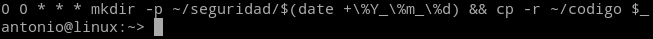
\includegraphics[width=1\textwidth]{imagenes/cron}
    \caption{Comando insertado en crontab para realizar una copia de seguridad diaria.}
    \label{fig1}
  \end{center}
\end{figure}

\subsection{Analizando qué ocurre en el kernel con DMESG}


\subsubsection{Cuestión 3}
\textit{Pruebe a ejecutar el comando, conectar un dispositivo USB y vuelva a ejecutar el comando. Copie y pegue la salida del comando. (considere usar dmesg | tail). Comente qué observa en la información mostrada.}
\newline

Al ejecutar el comando por promera vez obtenemos la informacion mostrada en la  \cref{fig2}, tras insertar un dispositivo USB, la información mostrada cambia como se muestra en la  \cref{fig3}. En esta informacion se muestran datos acerca del dispositivo UBS conectado, entre los que se incluyen el nombre del producto, el fabricante y el numero de serie entre otros.
\begin{figure}[H]
  \begin{center}
    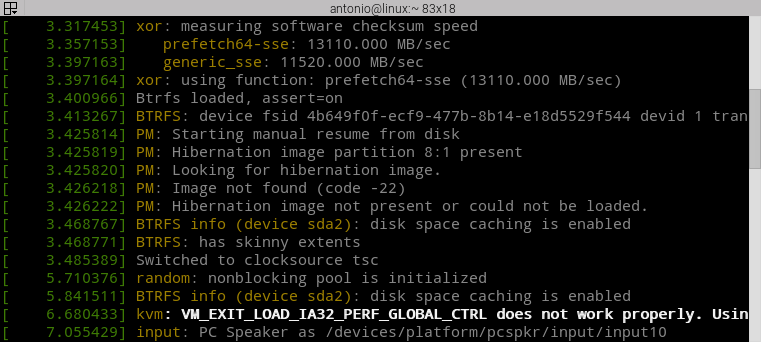
\includegraphics[width=1\textwidth]{imagenes/dmesg1}
    \caption{Ejecución de dmesg antes de insertar un USB.}
    \label{fig2}
  \end{center}
\end{figure}
\begin{figure}[H]
  \begin{center}
    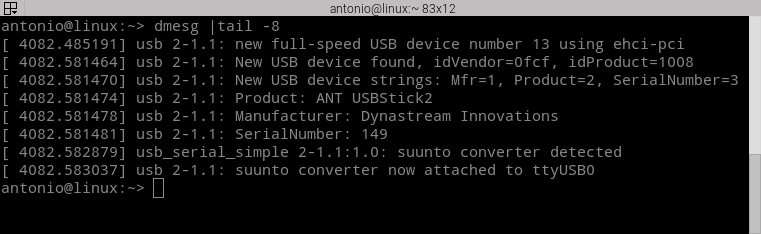
\includegraphics[width=1\textwidth]{imagenes/dmesg2}
    \caption{Ejecución de dmesg tras la conexión de un dispositivo USB.}
    \label{fig3}
  \end{center}
\end{figure}

\section{Monitorizando Windows: PERFMON}
\subsection{Cuestión 4}
\textit{Ejecute el monitor de “System Performance” y muestre el resultado. Incluya capturas de pantalla comentando la información que aparece.}
\newline

Al ejecutar el monitor “System Performance” por primera vez, se obtiene una pantalla como la mostrada en la  \cref{fig4}, en la que aparecen varias cosas: a la izquierda, tenemos un menú para realizar diferentes tareas con el monitor, en la parte central de la pantalla aparecen tres cuadros, dos de ellos para obtener información y uno con un resumen del sistema en el que se muestran estadísticas sobre el disco duro, el procesador,la red y la memoria RAM.

\begin{figure}[H]
  \begin{center}
    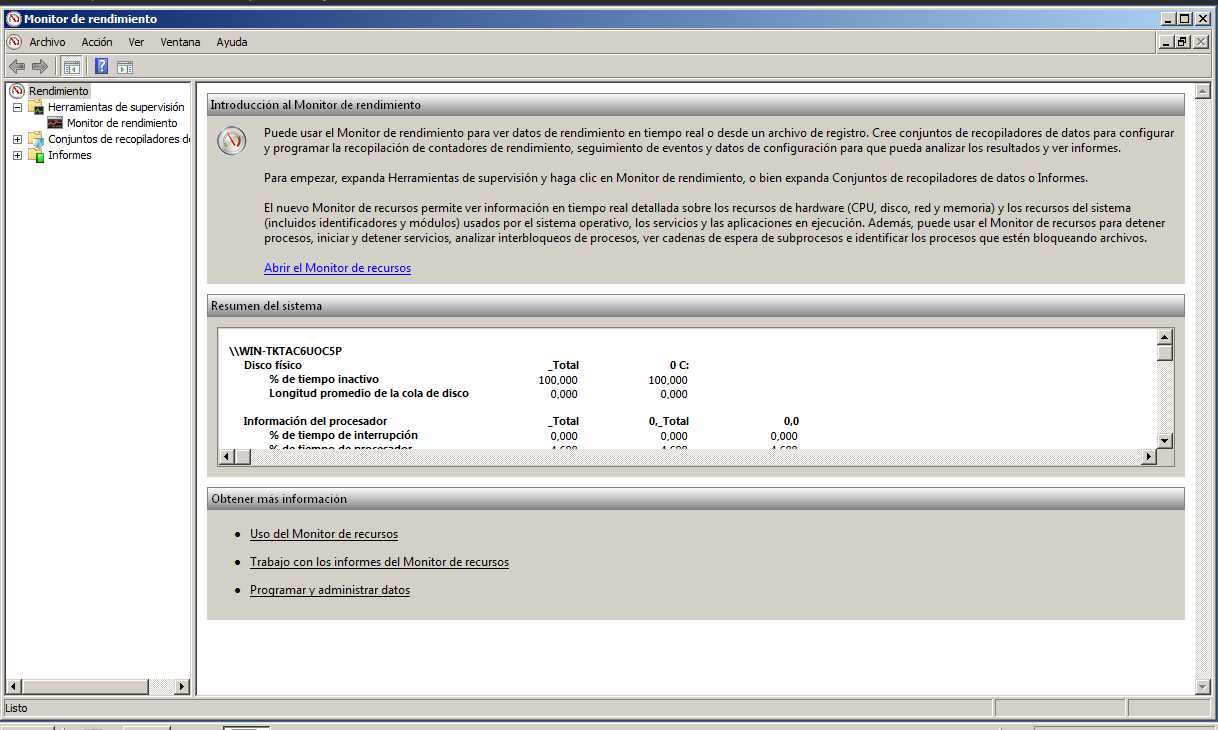
\includegraphics[width=1\textwidth]{imagenes/perfmon}
    \caption{Pantalla inicial de “System Performance”.}
    \label{fig4}
  \end{center}
\end{figure}

\subsection{Cuestión 5}
\textit{Cree un recopilador de datos definido por el usuario (modo avanzado) que incluya tanto el contador de rendimiento como los datos de seguimiento:Todos los referentes al procesador, al proceso y al servicio web. Intervalo de muestra 15 segundos. Almacene el resultado en el directorio Escritorio\\logs Incluya las capturas de pantalla de cada paso.}
\newline

El proceso para la creación de un recopilador de datos con las características citadas en la cuestión, se puede ver en en las \crefrange{fig5}{fig12}.

\begin{figure}[H]
  \begin{center}
    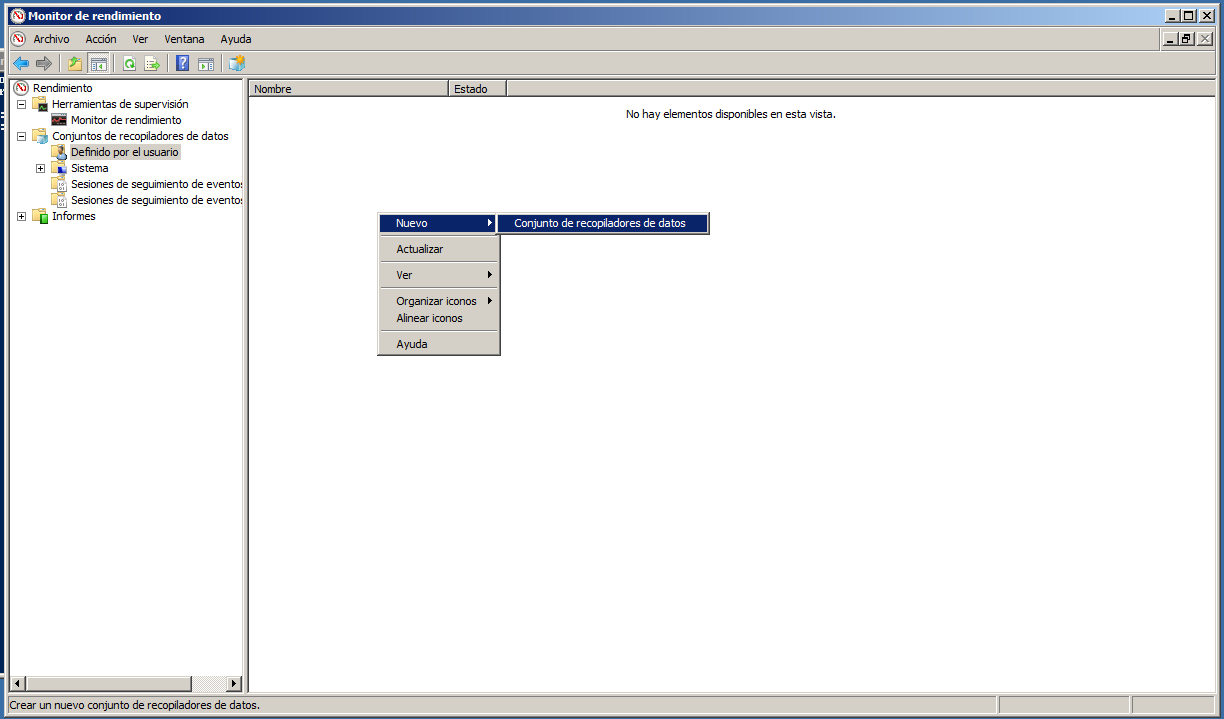
\includegraphics[width=1\textwidth]{imagenes/rec1}
    \caption{Panatalla para empezar a crear un nuevo recopilador.}
    \label{fig5}
  \end{center}
\end{figure}

\begin{figure}[H]
  \begin{center}
    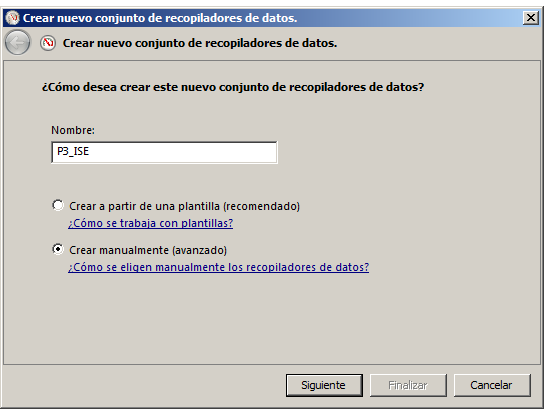
\includegraphics[width=0.7\textwidth]{imagenes/rec2}
    \caption{Selección del nombre y la forma de creación del recopilador”.}
    \label{fig6}
  \end{center}
\end{figure}

\begin{figure}[H]
  \begin{center}
    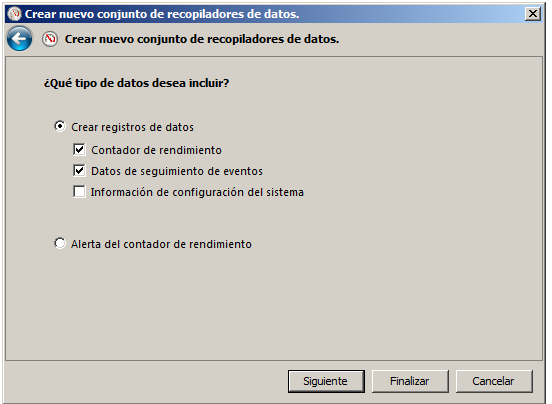
\includegraphics[width=0.7\textwidth]{imagenes/rec3}
    \caption{Pantalla para seleccionar que datos se desean incluir.}
    \label{fig7}
  \end{center}
\end{figure}

\begin{figure}[H]
  \begin{center}
    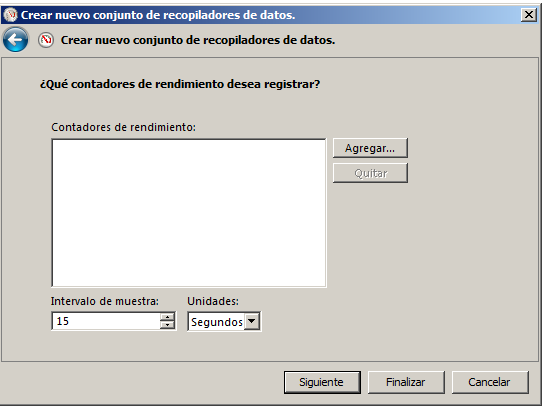
\includegraphics[width=0.7\textwidth]{imagenes/rec3_5}
    \caption{Pantalla para agregar contadores de rendimiento}
    \label{fig8}
  \end{center}
\end{figure}

\begin{figure}[H]
  \begin{center}
    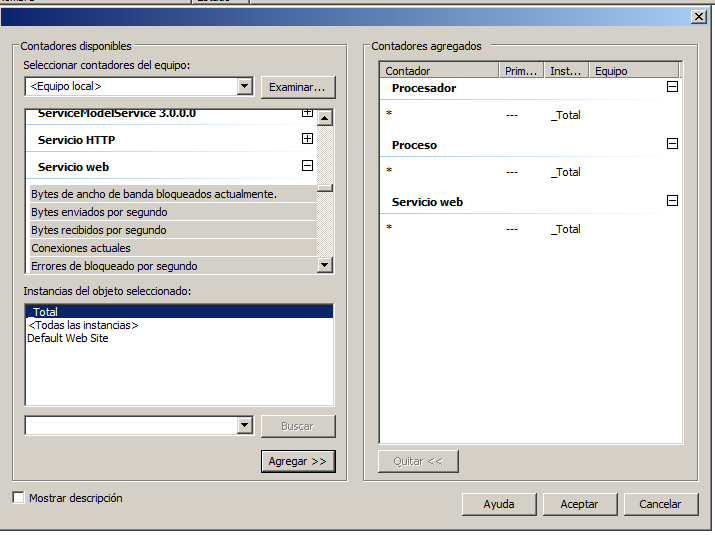
\includegraphics[width=0.7\textwidth]{imagenes/rec4}
    \caption{Proceso para seleccionar los contadores de rendimiento que se quieren añadir.}
    \label{fig9}
  \end{center}
\end{figure}

\begin{figure}[H]
  \begin{center}
    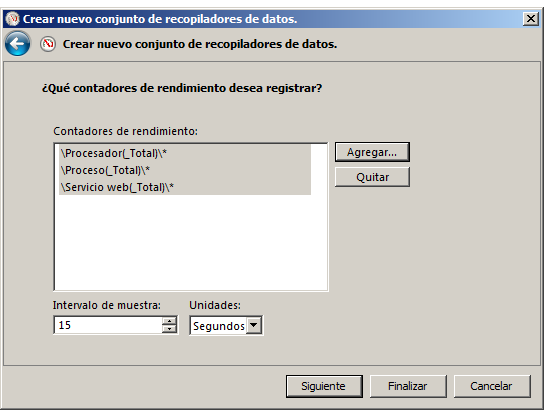
\includegraphics[width=0.7\textwidth]{imagenes/rec5}
    \caption{Pantalla con los contadores de rendimiento seleccionados.}
    \label{fig10}
  \end{center}
\end{figure}

\begin{figure}[H]
  \begin{center}
    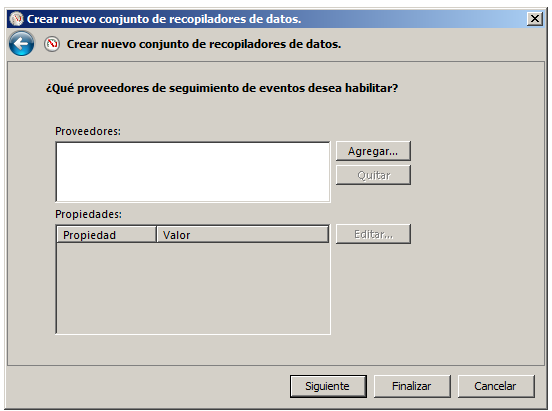
\includegraphics[width=0.7\textwidth]{imagenes/rec6}
    \caption{Pantalla para seleccionar proveedores de seguimiento.}
    \label{fig11}
  \end{center}
\end{figure}

\begin{figure}[H]
  \begin{center}
    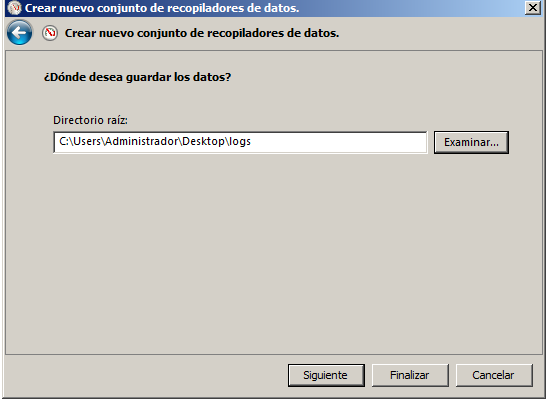
\includegraphics[width=0.7\textwidth]{imagenes/rec7}
    \caption{Pantalla para indicar la ruta donde se guardaran los datos.}
    \label{fig12}
  \end{center}
\end{figure}



\section{Monitorizando el hardware}
\subsection{Cuestión 6}
\textit{Instale alguno de los monitores comentados arriba en su máquina y pruebe a ejecutarlos (tenga en cuenta que si lo hace en la máquina virtual, los resultados pueden no ser realistas). Alternativamente, busque otros monitores para hardware comerciales o de código abierto para Windows y Linux.}
\newline

Para este apartado he instalado los monitores lm-sensors y hddtemp, usando el comando mostrado en la  \cref{fig13}. Los resultados de la ejecución muestran datos sobre la temperatura y los voltajes, como se muestra en las s \ \crefrange{fig14}{fig15}.
\begin{figure}[H]
  \begin{center}
    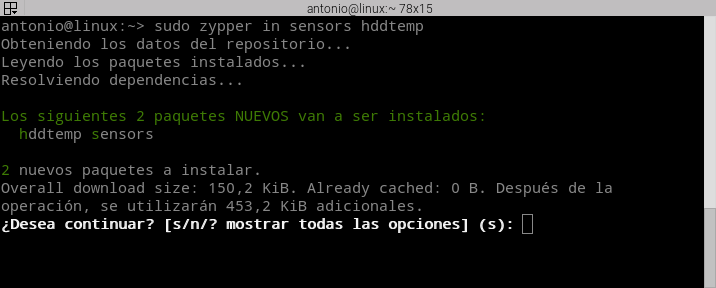
\includegraphics[width=1\textwidth]{imagenes/sensors}
    \caption{Instalación de los monitores hddtemp y lm-sensors en OpenSuse.}
    \label{fig13}
  \end{center}
\end{figure}

\begin{figure}[H]
    \centering
    \begin{subfigure}[b]{0.55\textwidth}
        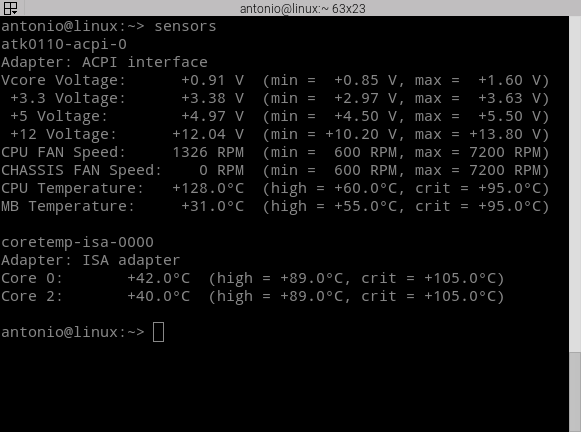
\includegraphics[width=\textwidth]{imagenes/sensors2}
        \caption{Ejecución de lm-sensors.}
        \label{fig14}
    \end{subfigure}
    \begin{subfigure}[b]{0.4\textwidth}
        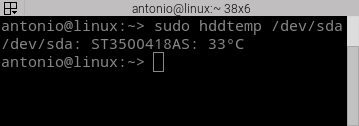
\includegraphics[width=\textwidth]{imagenes/hddtemp}
        \caption{Ejecución de hddtemp.}
        \label{fig15}
    \end{subfigure}
    \caption{Ejecución monitores lm-sensors y hddtemp.}
\end{figure}

\section{Otros monitores del sistema}
\subsection{MUNIM}


\subsubsection{Cuestión 7}
\textit{Visite la web del proyecto y acceda a la demo que proporcionan (http://demo.munin-monitoring.org/) donde se muestra cómo monitorizan un servidor. Monitorice varios parámetros y haga capturas de pantalla de lo que está mostrando comentando qué observa.}
\subsection{NAGIOS}


\subsubsection{Cuestión opcional 2}
\textit{Instale Nagios en su sistema (el que prefiera) documentando el proceso y muestre el resultado de la monitorización de su sistema comentando qué aparece.}
\subsection{GANGLIA}


\subsubsection{Cuestión opcional 3}
\textit{Haga lo mismo que con Munin.}
\subsection{ZABBIX}


\subsubsection{Cuestión opcional 4}
\textit{Prueba a instalar este monitor es alguno de sus tres sistemas. Realice capturas de pantalla del proceso de instalación y comente capturas de pantalla del programa en ejecución.}
\subsection{CACTI}


\subsubsection{Cuestión opcional 5}
\textit{Pruebe a instalar este monitor es alguno de sus tres sistemas. Realice capturas de pantalla del proceso de instalación y comente capturas de pantalla del programa en ejecución.}
\subsection{AWSTATS}


\subsubsection{Cuestión opcional 6}
\textit{Instale el monitor y muestre y comente algunas capturas de pantalla.}
\subsection{Monitorizando un servicio (o ejecución de un programa)}

\subsubsection{Cuestión 8}
\textit{Escriba un breve resumen sobre alguno de los artículos donde se muestra el uso de strace o busque otro y coméntelo.}
\section{Profiling}
\subsection{GPROF Y VALGRIND}


\subsubsection{Cuestión opcional 7}
\textit{Desarrolle una página en C o C++ y analice su comportamiento usando valgrind. Visite http://www.cs.tut.fi/~jkorpela/forms/cgic.html para ver un ejemplo sencillo de una página web generada por un programa escrito en C.}
\subsection{PHP}


\subsubsection{Cuestión opcional 8}
\textit{Desarrolle un script en PHP y analice su ejecución con alguno (o los dos) profilers.}
\subsection{PYTHON}



\subsubsection{Cuestión opcional 9}
\textit{Escriba un script en python y analice su comportamiento usando el profiler presentado.}

\subsection{POWERSHELL}


\subsubsection{Cuestión opcional 10}
\textit{Escriba un script en PowerShell y analice su comportamiento usando el profiler presentado.}
\subsection{MySQL}



\subsubsection{Cuestión 9}
\textit{Acceda a la consola mysql (o a través de phpMyAdmin) y muestre el resultado de mostrar el ”profile” de una consulta (la creación de la BD y la consulta la puede hacer líbremente).}
\subsection{MongoDB}


\subsubsection{Cuestión opcional 11}
\textit{Al igual que ha realizado el “profiling” con MySQL, realice lo mismo con MongoDB y compare los resultados (use la misma información y la misma consulta, hay traductores de consultas SQL a Mongo).}

%*************************************************************
\newpage
\bibliographystyle{ieeetr}
\bibliography{citas}

\end{document}
